\documentclass[aspectratio=169,10pt]{beamer}

% ---------- Style ----------
\usetheme{Madrid}
\usecolortheme{seahorse}
\setbeamertemplate{navigation symbols}{}
\setbeamertemplate{caption}[numbered]
\setbeamertemplate{itemize item}{\raise0.2ex\hbox{\scriptsize$\blacktriangleright$}}
\setbeamertemplate{itemize subitem}{\raise0.2ex\hbox{\tiny$\bullet$}}
\definecolor{deepblue}{RGB}{30,60,120}
\definecolor{softblue}{RGB}{235,242,252}
\setbeamercolor{title}{fg=deepblue}
\setbeamercolor{frametitle}{fg=deepblue,bg=softblue}
\setbeamercolor{structure}{fg=deepblue}
\setbeamerfont{frametitle}{series=\bfseries,size=\large}
\setbeamerfont{title}{series=\bfseries,size=\Large}

% ---------- Packages ----------
\usepackage[utf8]{inputenc}
\usepackage[T1]{fontenc}
\usepackage{amsmath,amssymb,bm}
\usepackage{booktabs}
\usepackage{array}
\usepackage{graphicx}
\usepackage{multicol}
\usepackage{mathtools}
\usepackage{ragged2e}
\graphicspath{{figures/}}

% ---------- Short commands ----------
\newcommand{\R}{\mathbb{R}}
\newcommand{\dd}{\mathrm{d}}
\newcommand{\eig}{\lambda_{\mathrm{eig}}}
\newcommand{\state}{(S,x,y,z)}
\newcommand{\smallnote}[1]{\vspace{0.3em}{\scriptsize\color{gray!70!black}#1}}

% ---------- Title ----------
\title[Chemostat Food Chain]{Stability and Bifurcation of a Simple Food Chain in a Chemostat with Removal Rates}
\subtitle{Mathematical Modelling Project Presentation}
\author[Group 4]{Nguyen Cong Hung \and Nguyen Tran Minh Tri \and Bui Huu Vinh \and Ngo Quang Duc \and Pham Chi Bang}
\institute[HUST]{School of Information and Communications Technology\\Hanoi University of Science and Technology}
\date{June 2026}

\begin{document}

% 1
\begin{frame}
  \titlepage
  \vspace{-1.5em}
  \begin{center}
    
\includegraphics[height=0.7cm]{p01_img1.png}
  \end{center}
\end{frame}

% 2
\begin{frame}{Presentation Roadmap}
\begin{columns}[T,onlytextwidth]
\column{0.52\textwidth}
\begin{enumerate}
  \item Biological motivation
  \item Mathematical model
  \item Equilibria and stability
  \item Numerical evidence
\end{enumerate}
\column{0.45\textwidth}
\begin{enumerate}\setcounter{enumi}{4}
  \item Persistence and coexistence
  \item Hopf bifurcation
  \item Effect of removal rates
  \item Main conclusion
\end{enumerate}
\end{columns}
\vspace{0.7em}
\begin{block}{Core message}
Distinct removal rates change the qualitative long-run behavior of the food chain.
\end{block}
\end{frame}

% 3
\begin{frame}{Problem and Key Question}
\begin{block}{Biological setting}
A chemostat continuously adds nutrient and removes culture medium, keeping volume approximately constant.
\end{block}
\vspace{0.4em}
\begin{columns}[T,onlytextwidth]
\column{0.48\textwidth}
\textbf{Food chain}
\[
S \longrightarrow x \longrightarrow y \longrightarrow z
\]
\begin{itemize}
  \item $S$: nutrient
  \item $x$: prey
  \item $y,z$: first and second predators
\end{itemize}
\column{0.48\textwidth}
\textbf{Main question}
\begin{itemize}
  \item Which species survive?
  \item When is coexistence stable?
  \item When do oscillations appear?
  \item How do $D_1,D_2,D_3$ reshape the outcome?
\end{itemize}
\end{columns}
\end{frame}

% 4
\begin{frame}{State Variables and Biological Meaning}
\centering
\renewcommand{\arraystretch}{1.25}
\begin{tabular}{c p{0.33\textwidth} p{0.36\textwidth}}
\toprule
Symbol & Meaning & Role \\
\midrule
$S(t)$ & Nutrient concentration & Resource consumed by prey \\
$x(t)$ & Prey population & Consumes nutrient \\
$y(t)$ & First predator & Consumes prey \\
$z(t)$ & Second predator & Consumes first predator \\
$D_i$ & Removal rates & Species-specific loss rates \\
\bottomrule
\end{tabular}
\vspace{1em}
\begin{block}{Feasible state space}
\[
S(t),x(t),y(t),z(t) \ge 0.
\]
\end{block}
\end{frame}

% 5
\begin{frame}{Model Equations}
\begin{align*}
\frac{\dd S}{\dd t} &= 1-S-f_1(S)x,\\
\frac{\dd x}{\dd t} &= x\bigl(f_1(S)-D_1\bigr)-f_2(x)y,\\
\frac{\dd y}{\dd t} &= y\bigl(f_2(x)-D_2\bigr)-f_3(y)z,\\
\frac{\dd z}{\dd t} &= z\bigl(f_3(y)-D_3\bigr).
\end{align*}
\vspace{-0.2em}
\begin{columns}[T,onlytextwidth]
\column{0.49\textwidth}
\begin{itemize}
  \item $1-S$: nutrient inflow and washout
  \item $f_1(S)x$: nutrient consumed by prey
\end{itemize}
\column{0.49\textwidth}
\begin{itemize}
  \item $D_i$: removal of population $i$
  \item $f_i$: biological response rate
\end{itemize}
\end{columns}
\end{frame}

% 6
\begin{frame}{Response Functions}
\begin{block}{General assumptions}
\[
f_i(0)=0, \qquad f_i\in C^1, \qquad f_i'(u)>0 \quad (u>0).
\]
\end{block}
\vspace{0.5em}
\begin{block}{Monod-type functions used in simulations}
\[
f_1(S)=\frac{a_1S}{b_1+S},\qquad
f_2(x)=\frac{a_2x}{b_2+x},\qquad
f_3(y)=\frac{a_3y}{b_3+y}.
\]
\end{block}
\begin{itemize}
  \item Increasing response with saturation.
  \item Biologically interpretable parameters: $a_i$ controls maximum response, $b_i$ controls half-saturation.
\end{itemize}
\end{frame}

% 7
\begin{frame}{Why Distinct Removal Rates Matter}
Adding the four equations gives
\[
\frac{\dd}{\dd t}(S+x+y+z)=1-S-D_1x-D_2y-D_3z.
\]
\vspace{0.3em}
\begin{columns}[T,onlytextwidth]
\column{0.49\textwidth}
\begin{block}{If removal rates were identical}
A simpler total-quantity relation could be used to reduce the system.
\end{block}
\column{0.49\textwidth}
\begin{alertblock}{With distinct removal rates}
The right-hand side depends on $x,y,z$ separately. The full four-dimensional system must be studied.
\end{alertblock}
\end{columns}
\vspace{0.6em}
\centering
\Large $D_1\neq D_2\neq D_3 \quad \Rightarrow \quad$ richer dynamics
\end{frame}

% 8
\begin{frame}{Numerical Workflow}
\begin{columns}[T,onlytextwidth]
\column{0.55\textwidth}
\begin{enumerate}
  \item Choose Monod response functions.
  \item Set parameter values and initial condition.
  \item Solve ODEs using adaptive Runge-Kutta.
  \item Discard transient behavior.
  \item Classify long-run regime.
\end{enumerate}
\column{0.42\textwidth}
\begin{block}{Observed regimes}
\begin{itemize}
  \item Washout
  \item Prey-only survival
  \item Boundary coexistence
  \item Stable coexistence
  \item Oscillatory coexistence
\end{itemize}
\end{block}
\end{columns}
\end{frame}

% 9
\begin{frame}{Positivity, Boundedness, and Dissipativity}
\begin{columns}[T,onlytextwidth]
\column{0.48\textwidth}
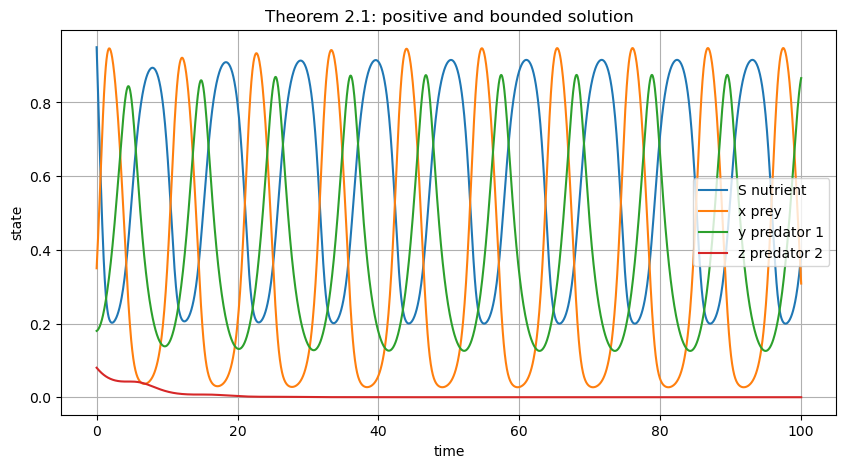
\includegraphics[width=\linewidth]{p08_img1.png}
\centering\scriptsize Positivity and Boundedness
\column{0.48\textwidth}
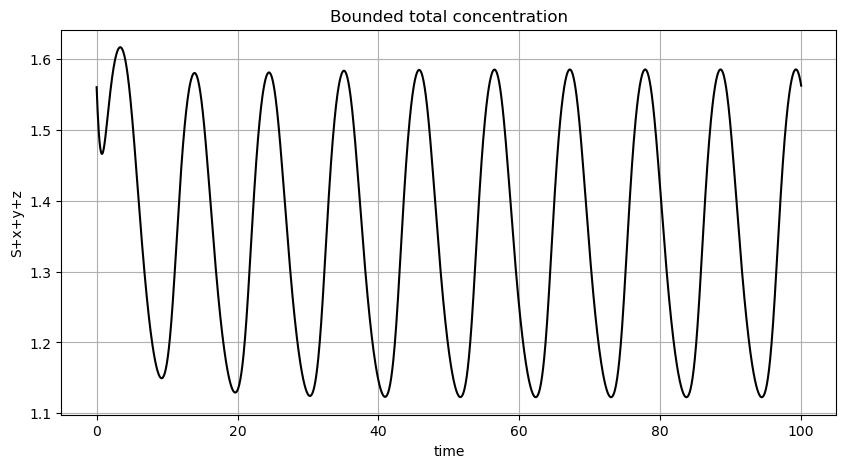
\includegraphics[width=\linewidth]{p09_img1.png}
\centering\scriptsize Total Quantity Bounded
\end{columns}
\vspace{0.6em}
\begin{itemize}
  \item Solutions remain non-negative and bounded: $\min(S,x,y,z)\approx 2.02\times 10^{-9}$.
  \item Total quantity does not diverge: $1.1228 \le S+x+y+z \le 1.6164$.
  \item This provides numerical evidence for dissipative behavior and biological feasibility.
\end{itemize}
\end{frame}

% 10
\begin{frame}{Equilibrium Points}
\centering
\renewcommand{\arraystretch}{1.35}
\begin{tabular}{c c p{0.43\textwidth}}
\toprule
Equilibrium & Form & Biological meaning \\
\midrule
$P_0$ & $(1,0,0,0)$ & Washout of all organisms \\
$P_1$ & $(S_1,x_1,0,0)$ & Prey survives; predators extinct \\
$P_2$ & $(S_2,x_2,y_2,0)$ & Prey and first predator survive \\
$P_3$ & $(S_3,x_3,y_3,z_3)$ & Full coexistence \\
\bottomrule
\end{tabular}
\vspace{0.8em}
\begin{block}{Interpretation}
Equilibria are not only algebraic solutions; they represent possible ecological outcomes.
\end{block}
\end{frame}

% 11
\begin{frame}{Boundary Regimes: Time-Series and Phase View}
\begin{columns}[T,onlytextwidth]
\column{0.33\textwidth}
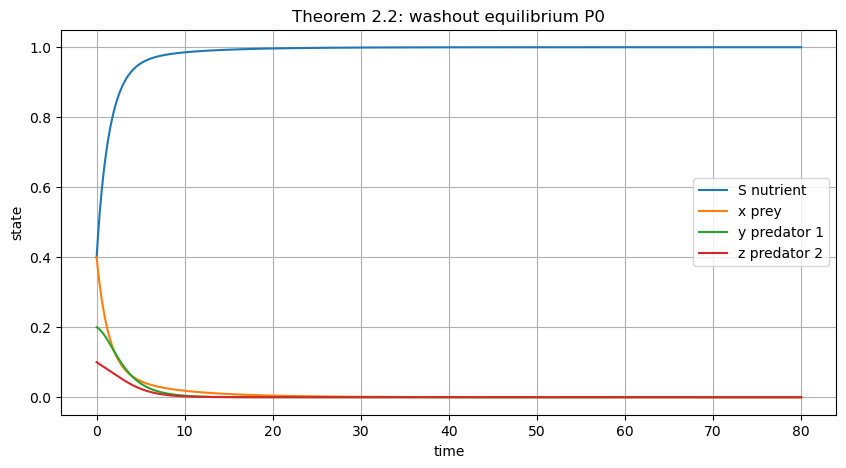
\includegraphics[width=\linewidth]{p11_img1.png}
\centering\scriptsize $P_0$: washout
\column{0.33\textwidth}
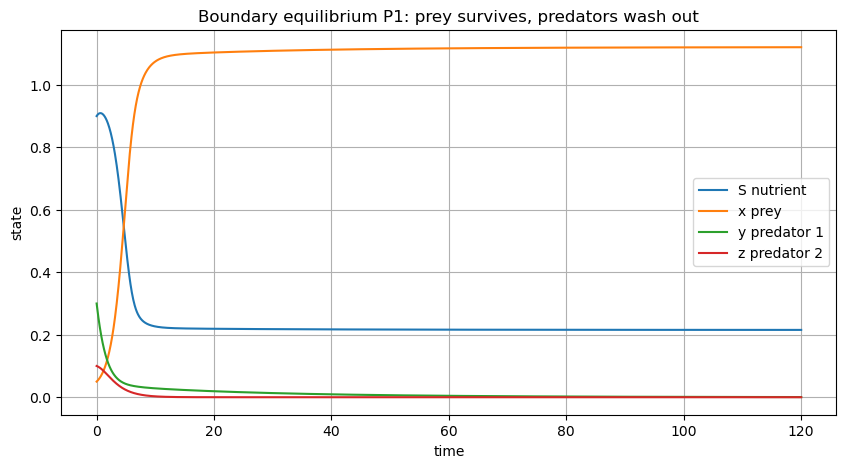
\includegraphics[width=\linewidth]{p11_img2.png}
\centering\scriptsize $P_1$: prey-only
\column{0.33\textwidth}
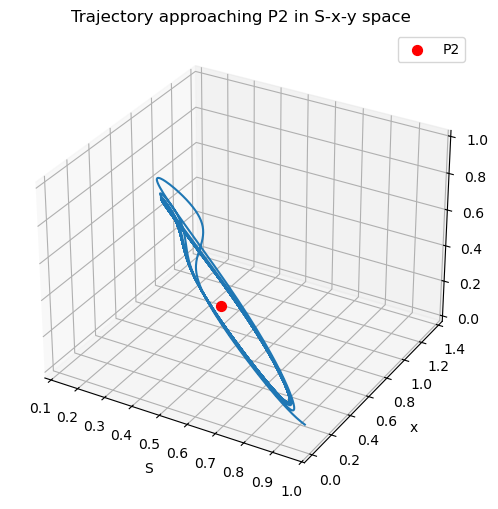
\includegraphics[width=\linewidth]{p11_img5.png}
\centering\scriptsize $P_2$: top predator washed out (phase view)
\end{columns}
\vspace{0.6em}
\begin{itemize}
  \item Different parameter conditions remove different trophic levels.
  \item Boundary equilibria correspond to real long-run regimes.
  \item Trajectories show attraction toward lower-dimensional ecological states.
\end{itemize}
\end{frame}

% 12
\begin{frame}{Local Stability and Boundary Checks}
\begin{block}{Linearization and Eigenvalue criterion}
\[
\max \operatorname{Re}(\eig)<0 \quad \Rightarrow \quad \text{locally asymptotically stable.}
\]
\end{block}
\vspace{0.5em}
\centering
\renewcommand{\arraystretch}{1.25}
\begin{tabular}{c p{0.32\textwidth} c p{0.25\textwidth}}
\toprule
Eq. & Main condition & Value & Interpretation \\
\midrule
$P_0$ & Prey invasion at nutrient-only state & $-0.1333$ & Washout stable \\
$P_1$ & First-predator invasion at prey-only state & $-0.0351$ & Prey-only survival \\
$P_2$ & Top-predator invasion $f_3(y_2)-D_3$ & $-0.1178$ & $z$ cannot persist \\
\bottomrule
\end{tabular}
\vspace{0.8em}
\begin{itemize}
  \item Invasion conditions are read from boundary eigenvalues.
  \item The $P_2$ value indicates the top predator cannot invade near that boundary state.
\end{itemize}
\end{frame}

% 13
\begin{frame}{Lyapunov Functions for Global Stability}
\begin{columns}[T,onlytextwidth]
\column{0.48\textwidth}
\begin{block}{Prey-only subsystem ($P_1$)}
\[
V(S,x)=\frac12(S-S_1)^2+\frac12(x-x_1)^2.
\]
\end{block}
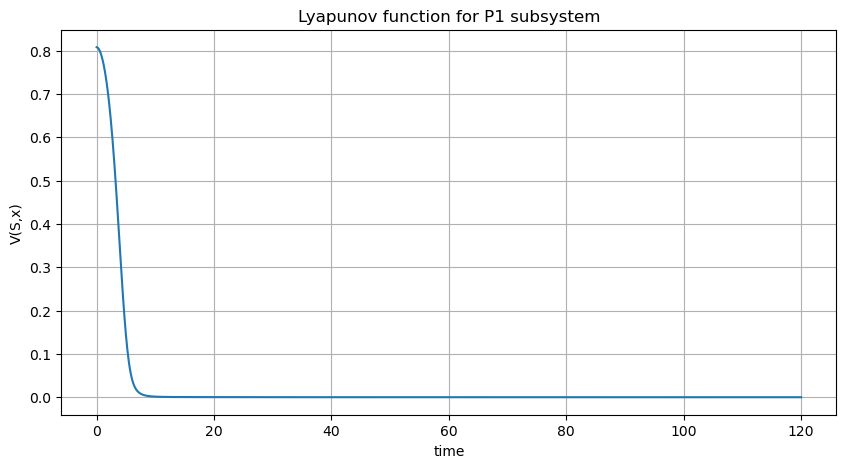
\includegraphics[width=\linewidth]{p14_img1.png}
\centering\scriptsize $V(S,x)$ near $P_1$
\column{0.48\textwidth}
\begin{block}{Boundary subsystem ($P_2$)}
\[
W(S,x,y)=S-S_2-S_2\ln\frac{S}{S_2}
+\frac12(x-x_2)^2+\frac12(y-y_2)^2.
\]
\end{block}
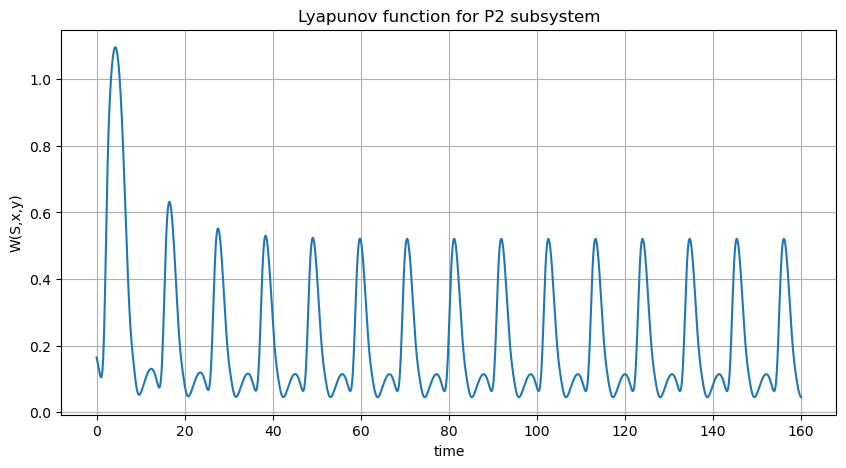
\includegraphics[width=\linewidth]{p14_img2.png}
\centering\scriptsize $W(S,x,y)$ near $P_2$
\end{columns}
\vspace{0.4em}
\begin{itemize}
  \item Profiles decrease toward small values, supporting global stability.
\end{itemize}
\end{frame}

% 14
\begin{frame}{Persistence and Coexistence at $P_3$}
\begin{columns}[T,onlytextwidth]
\column{0.48\textwidth}
\begin{block}{Coexistence equilibrium}
\[
P_3=(0.0669,1.6291,0.1667,0.3963).
\]
\end{block}
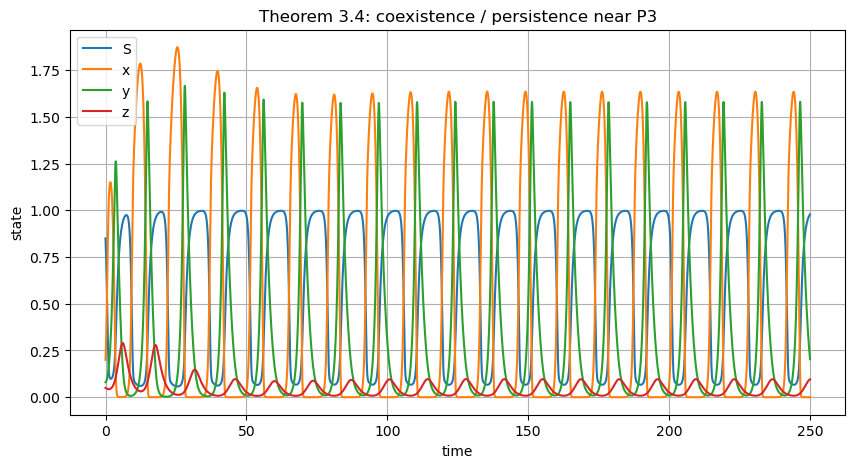
\includegraphics[width=0.85\linewidth]{p15_img1.png}
\centering\scriptsize Coexistence time series
\column{0.48\textwidth}
\begin{itemize}
  \item All four components are positive, meaning populations stay away from extinction.
  \item Behavior is robust across multiple positive initial conditions.
\end{itemize}
\vspace{0.5em}
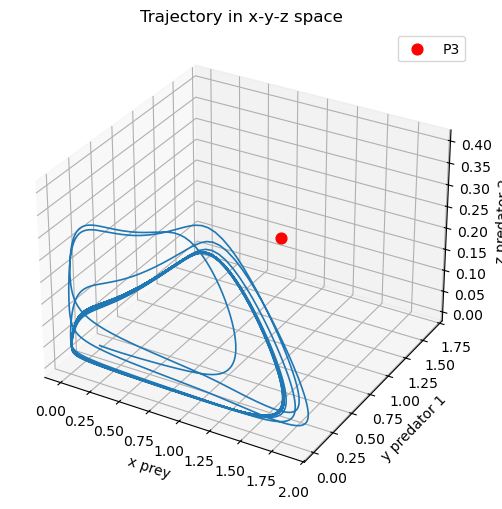
\includegraphics[width=0.85\linewidth]{p16_img1.png}
\centering\scriptsize Phase portrait near $P_3$
\end{columns}
\end{frame}

% 15
\begin{frame}{Hopf Bifurcation: Concept}
\begin{block}{Definition}
A Hopf bifurcation occurs when a complex conjugate pair of eigenvalues crosses the imaginary axis.
\end{block}
\[
\eig(\lambda)=\alpha(\lambda)\pm i\omega(\lambda),
\qquad \alpha(\lambda^*)=0,\quad \omega(\lambda^*)\ne 0.
\]
\vspace{0.4em}
\begin{columns}[T,onlytextwidth]
\column{0.48\textwidth}
\begin{itemize}
  \item Before crossing: equilibrium may be stable.
  \item After crossing: oscillations can appear.
\end{itemize}
\column{0.48\textwidth}
\begin{itemize}
  \item Ecological meaning: coexistence can be cyclic, not steady.
  \item Parameter used: $a_1=\lambda$.
\end{itemize}
\end{columns}
\end{frame}

% 16
\begin{frame}{Hopf Bifurcation Around $P_2$}
\begin{block}{Critical point: $\lambda^*\approx 9.6555,\quad \eig\approx\pm 1.6033i$}
Complex conjugate pair crosses the imaginary axis.
\end{block}
\vspace{0.4em}
\begin{columns}[T,onlytextwidth]
\column{0.48\textwidth}
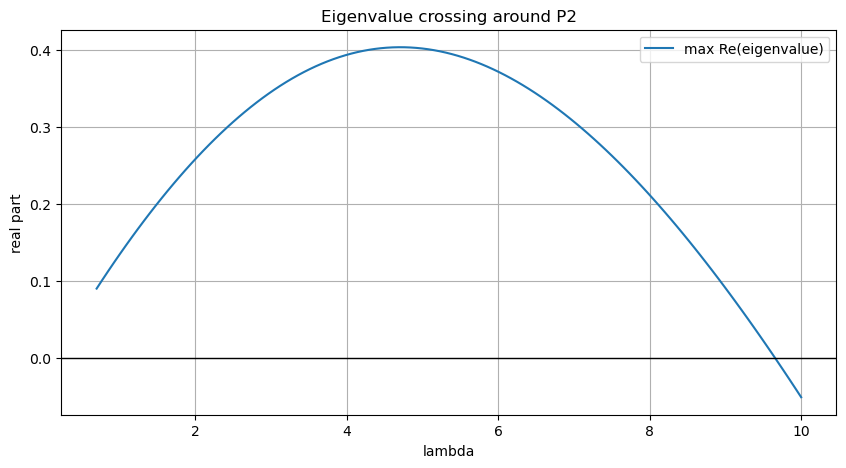
\includegraphics[width=0.85\linewidth]{p18_img1.png}
\centering\scriptsize Real part crossing
\column{0.48\textwidth}
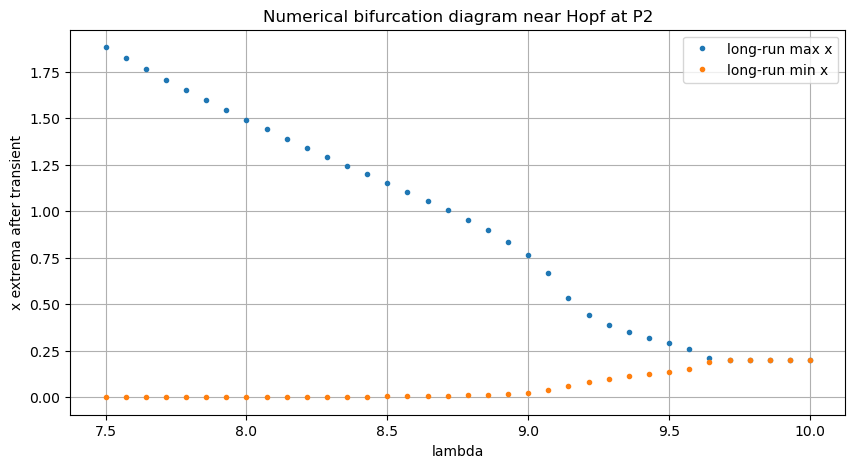
\includegraphics[width=0.85\linewidth]{p19_img3.png}
\centering\scriptsize Bifurcation diagram using $x(t)$ extrema
\end{columns}
\vspace{0.4em}
\begin{itemize}
  \item Split extrema indicate sustained boundary oscillation ($\lambda=8.5$).
  \item Coincident extrema indicate convergence to equilibrium ($\lambda=9.8$).
\end{itemize}
\end{frame}

% 17
\begin{frame}{Hopf Bifurcation Around $P_3$}
\begin{block}{Critical point: $\lambda^*\approx 2.9582,\quad \eig\approx\pm 0.4722i$}
All species can persist, but their densities may oscillate instead of settling to constants.
\end{block}
\vspace{0.4em}
\begin{columns}[T,onlytextwidth]
\column{0.32\textwidth}
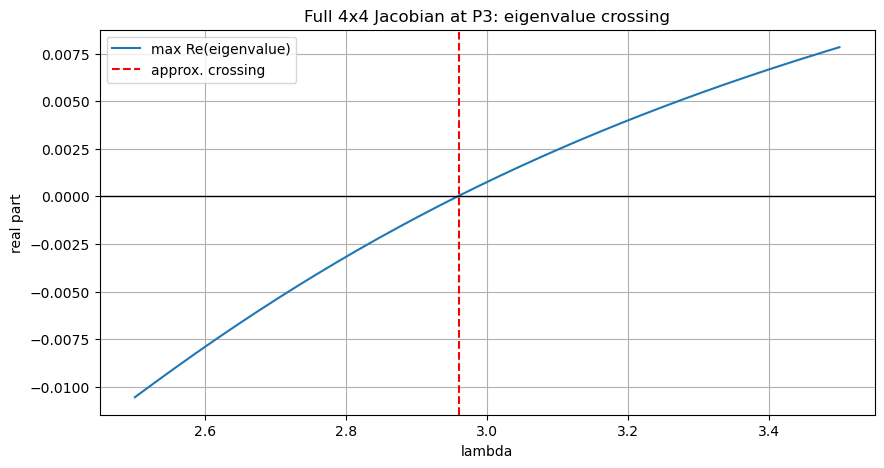
\includegraphics[width=\linewidth]{p20_img1.png}
\centering\scriptsize Real part crossing
\column{0.32\textwidth}
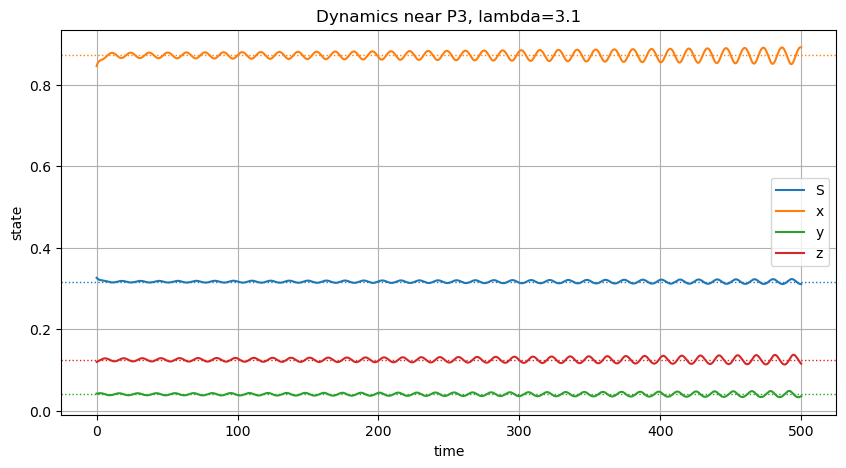
\includegraphics[width=\linewidth]{p21_img2.png}
\centering\scriptsize $\lambda=3.10$: oscillatory side
\column{0.32\textwidth}
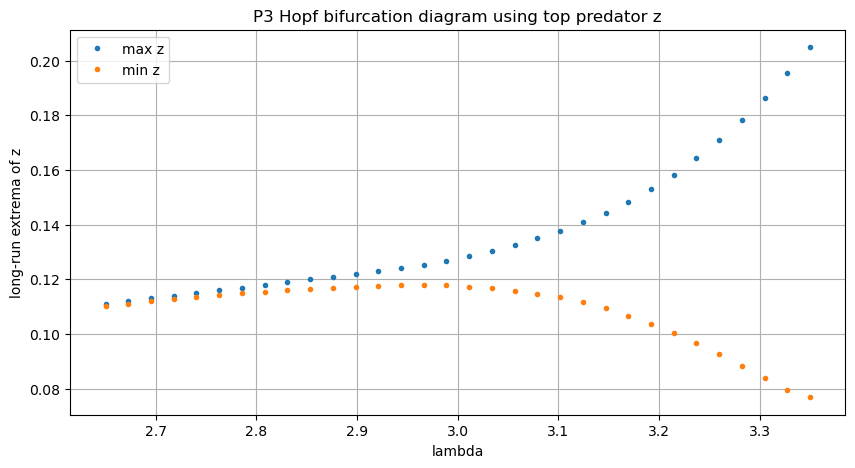
\includegraphics[width=\linewidth]{p22_img2.png}
\centering\scriptsize Top-predator extrema
\end{columns}
\end{frame}

% 18
\begin{frame}{Effect of Removal Rates: Phase Diagram}
\begin{columns}[T,onlytextwidth]
\column{0.5\textwidth}
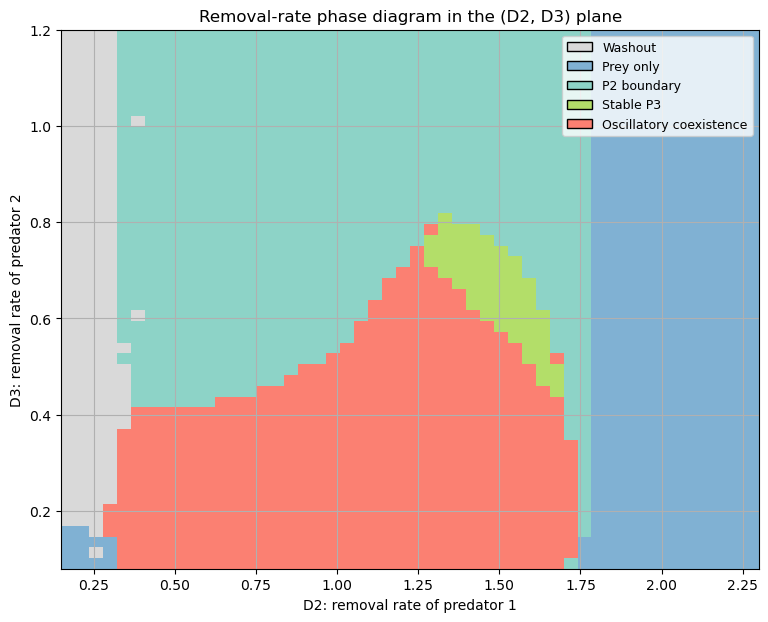
\includegraphics[width=\linewidth]{p23_img1.png}
\column{0.48\textwidth}
\begin{block}{Parameter sweep: $D_2\in[0.15,2.30],\quad D_3\in[0.08,1.20]$}
$D_2,D_3$ strongly shape survival and oscillation.
\end{block}
\vspace{0.5em}
\begin{columns}[T,onlytextwidth]
\column{0.48\textwidth}
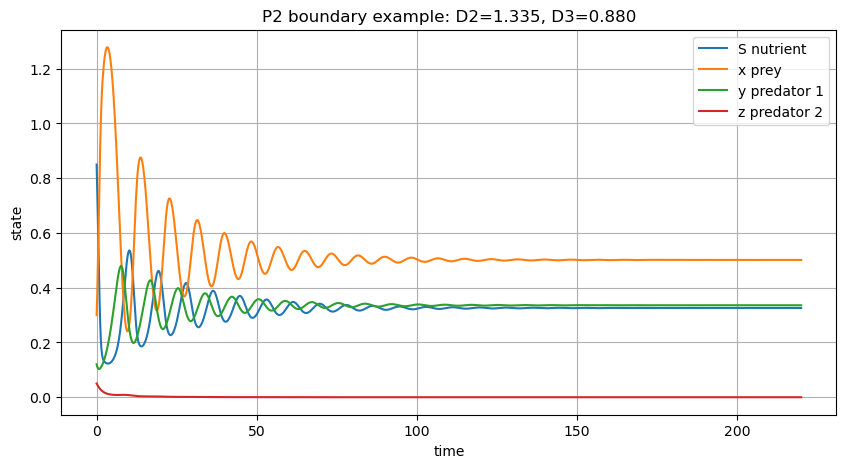
\includegraphics[width=\linewidth]{p25_img2.png}
\centering\scriptsize $P_2$ boundary
\column{0.48\textwidth}
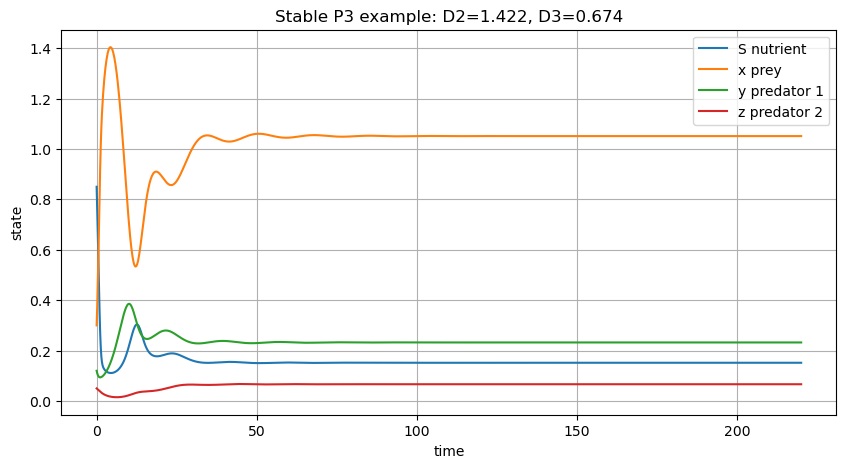
\includegraphics[width=\linewidth]{p25_img3.png}
\centering\scriptsize Stable $P_3$
\end{columns}
\begin{itemize}
  \item Large predator removal rates eliminate higher trophic levels.
\end{itemize}
\end{columns}
\end{frame}

% 19
\begin{frame}{Conclusion and Limitations}
\begin{columns}[T,onlytextwidth]
\column{0.53\textwidth}
\begin{block}{Main conclusions}
\begin{itemize}
  \item Positivity and boundedness are numerically supported.
  \item Boundary regimes match invasion conditions.
  \item Hopf bifurcation appears near both $P_2$ and $P_3$.
  \item Distinct removal rates reshape long-run ecological outcomes.
\end{itemize}
\end{block}
\column{0.43\textwidth}
\begin{alertblock}{Limitations}
\begin{itemize}
  \item No empirical calibration data.
  \item Deterministic model only.
  \item No delay, noise, space, or seasonality.
  \item Stability conditions may be sufficient, not necessary.
\end{itemize}
\end{alertblock}
\end{columns}
\vspace{0.5em}
\centering
\Large Distinct removal rates are mathematically and biologically meaningful.
\end{frame}

\end{document}
